\chapter{Introduction}

Cyber Physical Systems (CPS) are nowadays widely used in different application domains, such as smart-homes, smart-cities, hospitals, etc... They are mainly composed of two entities: a cyber part consisting in a computing and networking component, and a physical part consisting in different controllers and sensors. The existence of a connected cyber part implies its susceptibility to multiple cyber threats. The malfunctioning of these systems, due to a cyber threat, can cause severe impacts on the real life and the safety of the community, for example a blackout or water contamination. That is why many algorithms have been designed for the security monitoring of those systems, in particular the anomaly and attack detection.

Nowadays, machine and deep learning algorithms are used to detect those anomalies and intrusions. But, in majority, they rely only on the cyber part of the systems and on the data describing their behaviour, ignoring their physical models. The idea behind this work is to employ a hybrid machine learning algorithm, in particular neural networks, to detect anomalies and attacks in CPS considering its physical model.

In order to focus on the implementation of the hybrid machine learning algorithm, a CPS, with ready to use datasets, was chosen from a list provided in \cite{morris_industrial_nodate}: the power system \cite{adhikari_power_2014}, which network diagram was represented on figure \ref{fig:cps_rep}. The system is composed of two power generators who are alimenting the whole system. Intelligent Electronic Devices (IEDs) R1 to R4 and the breakers BR1 to BR4 can be found connected directly to those generators. Each IED switches its corresponding breaker when a fault is detected, valid or fake. The communication between the IEDs and the Substation Switch is done wirelessly. On the other hand the Substation Switch is connected with the Primary Domain Controller (PDC) and the Control Room.

\begin{figure}[H]
    \centering
    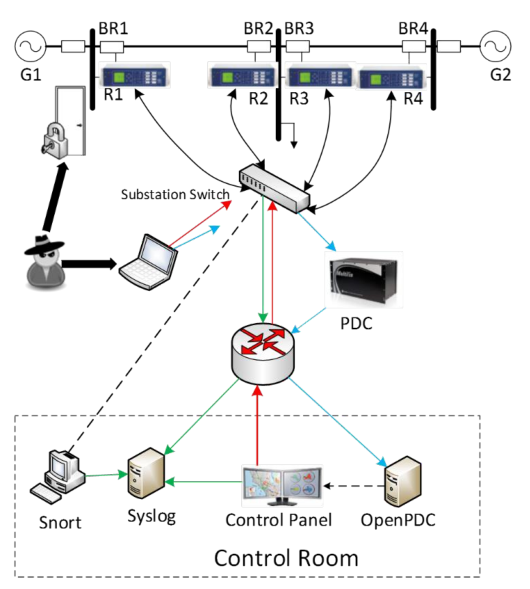
\includegraphics[width=100mm]{images/cps_rep.png}
    \caption{Power system network diagram \cite{adhikari_power_2014}}
    \label{fig:cps_rep}
\end{figure}

As mentioned before, the aim of the work is to fuse the black-box and theory-based models together to get better predictions. However this is not the first time such a fusion is examined. In the literature various approaches of the fusion of neural networks with theory-based models were presented. Those approaches can be divided into two types given what aspect of the algorithm they're changing: those that modify in first place the input to take into consideration the physical constraints, and those that modify the structure of the neural network.

-->here comes some more explanations--<

In the following chapters, it was decided to start with a less complex algorithms than neuron networks, so that the interpretation would be a lot simpler, in order to generalise the findings on the neural networks in further chapters. That is why the next chapter will talk about comparing some basic machine learning methods.